\section{Using the \textbf{TransP-0} design abstraction}
\label{demonstration}

In the following, we evaluate \textsc{TransP-0}. Therefore, we first present prototypical tool support in Section~\ref{tool}, which we have used for coding the actual system designs and optimizing their behavior. Then, we describe the sample system design in Section~\ref{examples}, which are intended to show the capabilities of the design abstraction. Finally, we discuss the results of and experiences made during the experiments in Section~\ref{discussion}. In particular, we are interested in the suitability of the design abstraction with respect to rapid and iterative design formulation as well as evaluation.

\subsection{Prototypical tool support}
\label{tool}

TODO

\begin{figure}[h]
	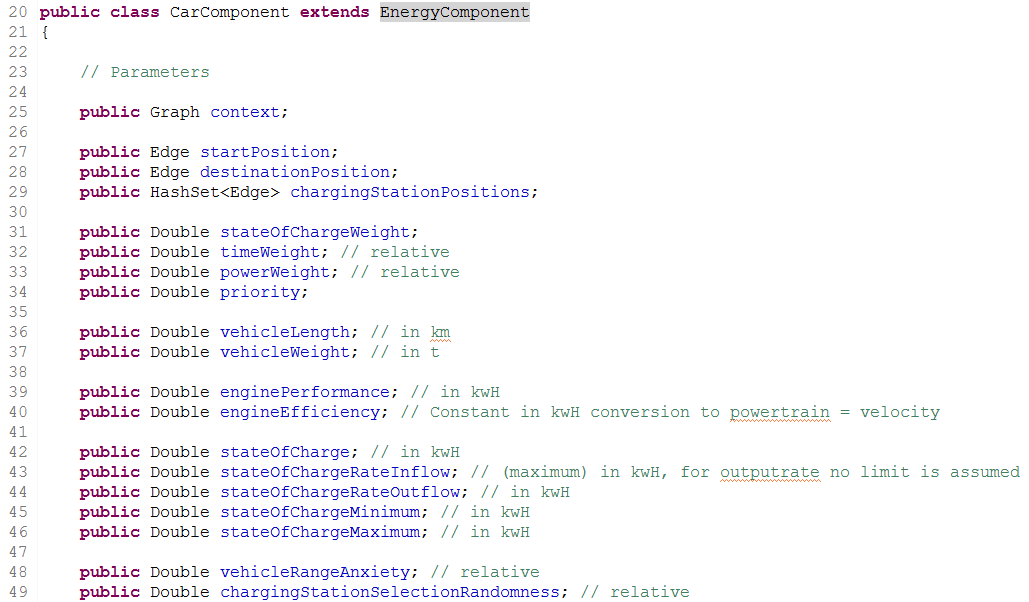
\includegraphics[width=\columnwidth]{./gfx/modeling.png}
	\caption{System modeling using regular Java classes and the Eclipse integrated development environment (IDE).}
	\label{figure:modeling}
\end{figure}

TODO

\begin{figure}[h]
	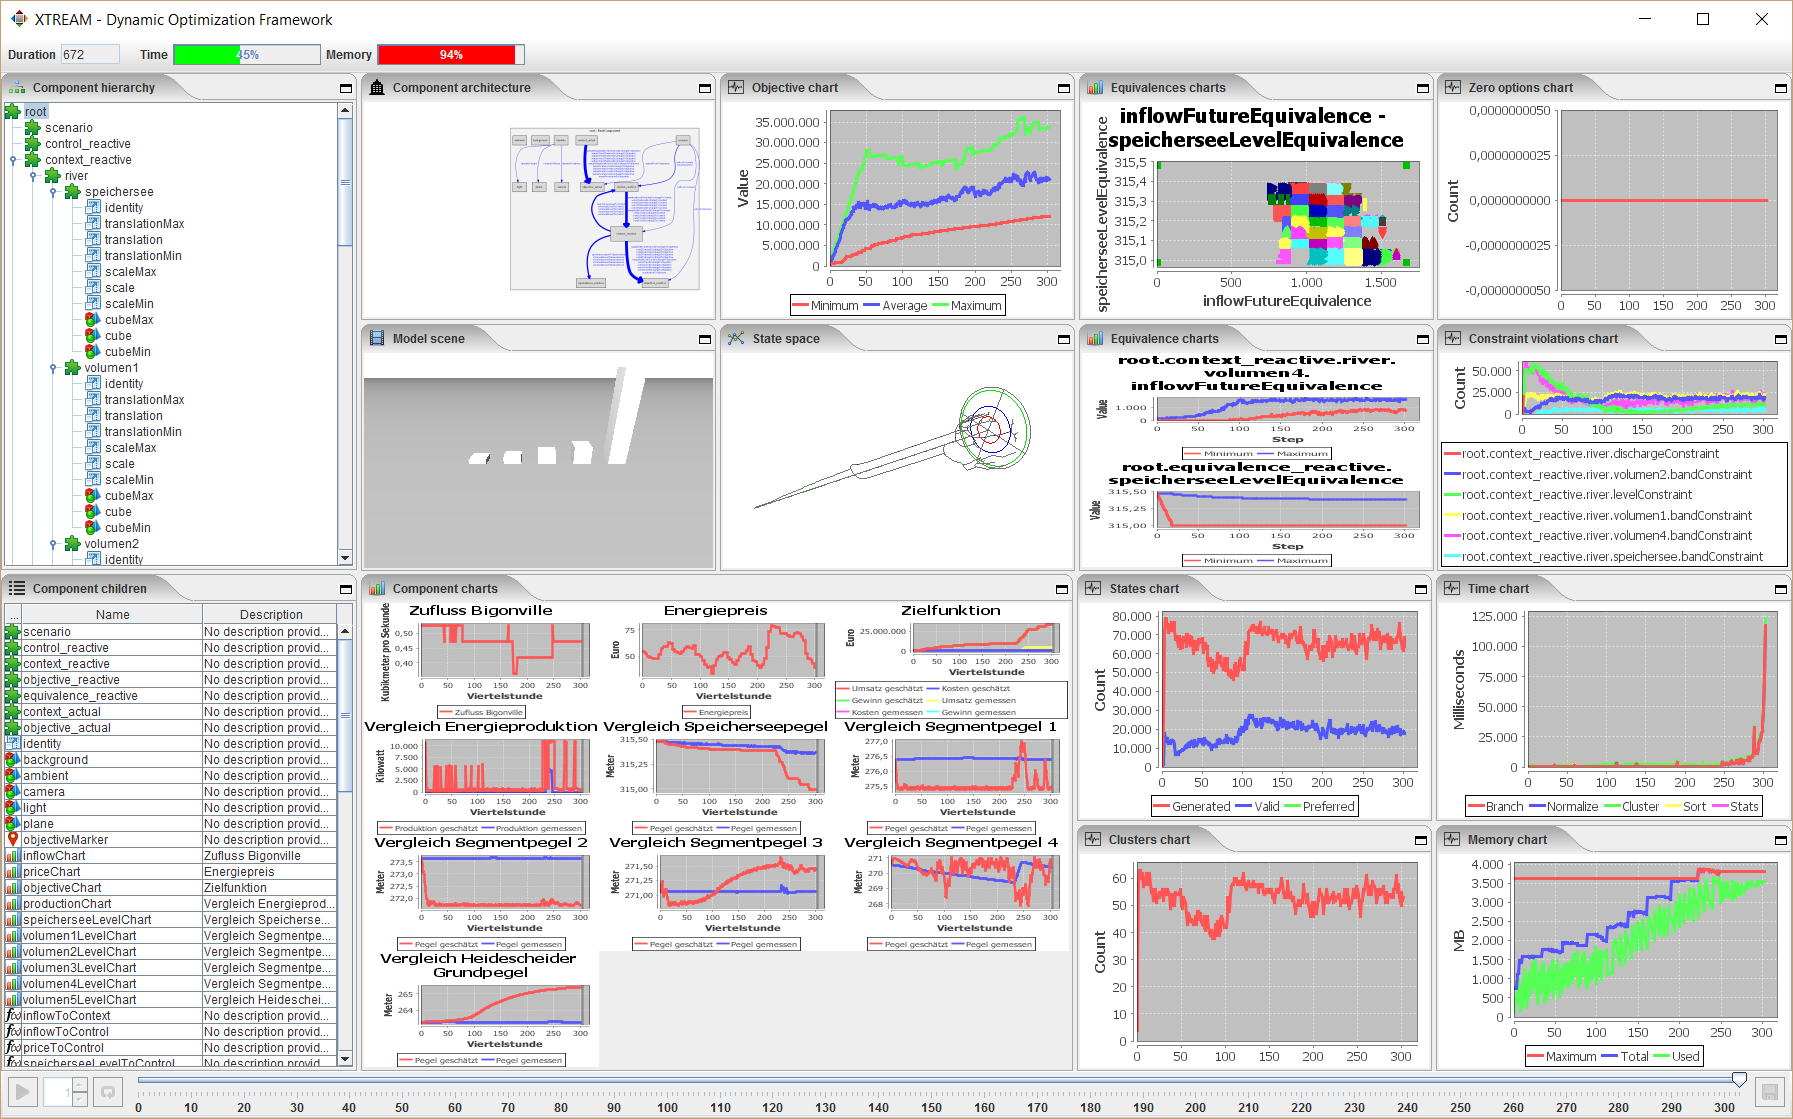
\includegraphics[width=\columnwidth]{./gfx/analysis.png}
	\caption{Model analysis using a basic approximate dynamic programming algorithm and comprehensive visualization techniques.}
	\label{figure:analysis}
\end{figure}

TODO

\subsection{Exemplary system designs}
\label{examples}

In this case study we propose a simple scenario for commuter traffic where ten traffic participants travel from home to work locations. In each time step traffic participants actions consist in selecting driving speed, time of charging, time of departure as well as route selection when driving towards their respective destination positions. The selected traffic infrastructure is consisted of a traffic network of 20 by 5 kilometers with two possible origins and two possible destinations of travel for individual traffic participants. 

\begin{figure}
	\centering
	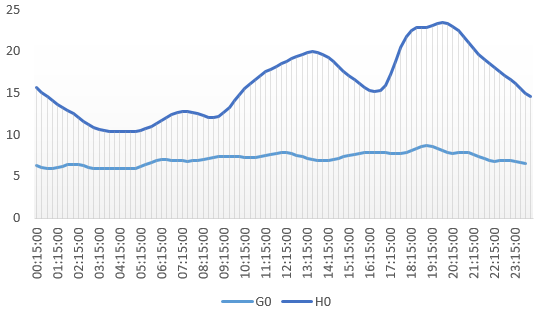
\includegraphics[width=\columnwidth]{gfx/profiles.PNG}
	\caption{Illustration of home (H0) and workplace (G0) load profiles.}
	\label{profiles}
\end{figure}

Subsequently, we evaluate traffic scenarios in terms of different configurations varying in their respective parameters. 

\subsubsection{Configuration 1: Objective function structure}

We consider three different scenarios when varying objective weight configuration: (1) focus on achieving energy-efficiency with regard to driving and power system balance, (2) focus on achieving shortest traveling time while driving as well as (3) an intermediate configuration of both energy-efficiency and shortest traveling time.

\subsubsection{Configuration 2: Voltage net structure}

We consider a changing voltage net structure within two configurations: (1) single voltage nets aggregating both the consumers and producers of home and workplaces as well as (2) allocation of two distinct voltage nets for the consumers and producers of home and workplaces. 

\subsubsection{Configuration 3: Traffic network structure}

Finally, we evaluate scenarios with regard to variation of the structure of the employed traffic network. Here, we vary the number of possible paths for traffic participants to travel from home to workplace destinations and vice versa.  

The results are pictured in Figure \ref{figure:examples}. 

\begin{table*}[b]
	\centering
	\renewcommand{\arraystretch}{1.3}
	\begin{tabularx}{\textwidth}{|Y|Y|Y|Y|}
		\hline
		
		\textbf{Scenario 1} & \textbf{Scenario 2} & \textbf{Scenario 3} \\
		
		\hline
		
		Energy-efficiency &
		Shortest traveling time &
		Intermediate \\
		
		\hline
		
		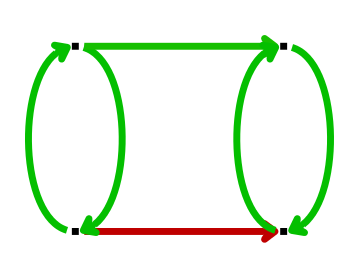
\includegraphics[width=0.20\textwidth, trim=0 0 0 -3]{gfx/Graph2.png} &
		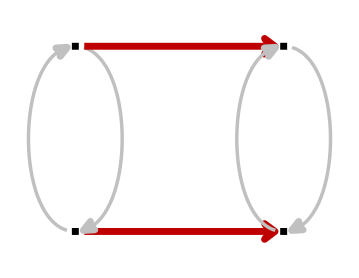
\includegraphics[width=0.20\textwidth, trim=0 0 0 -3]{gfx/Graph1.png} &
		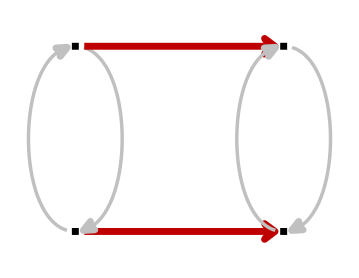
\includegraphics[width=0.20\textwidth, trim=0 0 0 -3]{gfx/Graph1.png} \\
		
		\hline
		
		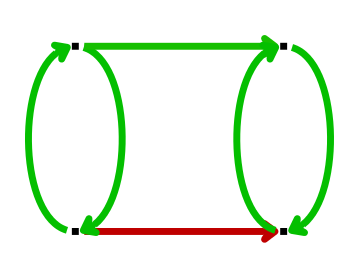
\includegraphics[width=0.20\textwidth, trim=0 0 0 -3]{gfx/Graph2.png} &
		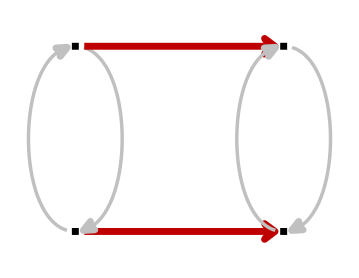
\includegraphics[width=0.20\textwidth, trim=0 0 0 -3]{gfx/Graph1.png} &
		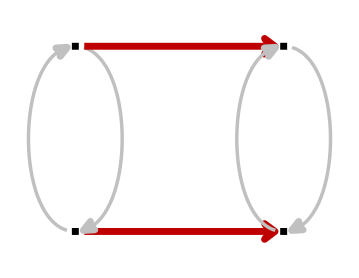
\includegraphics[width=0.20\textwidth, trim=0 0 0 -3]{gfx/Graph1.png} \\
		\hline			
	\end{tabularx}
	\caption{Traffic flow graph and power charts for different configurations.}
	\label{figure:examples}
\end{table*}